

\documentclass[journal]{IEEEtran}

\usepackage{cite}





% *** GRAPHICS RELATED PACKAGES ***
%
\ifCLASSINFOpdf
   \usepackage[pdftex]{graphicx}  
   %Please change to your image storage
   \graphicspath{{D:/githubfile/2021Operational-Statistics-SAR/Images/JPG/}}
   \DeclareGraphicsExtensions{.pdf,.jpeg,.png}
\else

\fi



\hyphenation{op-tical net-works semi-conduc-tor}


\begin{document}

\title{A Brief Group Introduction}


\author{Fanghan~Yang,~\IEEEmembership{Postgraduate,~XDU,}
        Zhaoji~Wu,~\IEEEmembership{Postgraduate,~XDU,}
        Xiyu~Fan,~\IEEEmembership{Postgraduate,~XDU,}
        and~Zhenhang~Weng,~\IEEEmembership{Postgraduate,~XDU}% <-this % stops a space
\thanks{M. Shell was with the Department
of Electrical and Computer Engineering, Georgia Institute of Technology, Atlanta,
GA, 30332 USA e-mail: (see http://www.michaelshell.org/contact.html).}% <-this % stops a space
\thanks{J. Doe and J. Doe are with Anonymous University.}% <-this % stops a space
\thanks{Manuscript received April 19, 2005; revised August 26, 2015.}}


% The paper headers
\markboth{Journal of \LaTeX\ Class Files,~Vol.~14, No.~8, August~2015}%
{Shell \MakeLowercase{\textit{et al.}}: Bare Demo of IEEEtran.cls for IEEE Journals}




% make the title area
\maketitle

% As a general rule, do not put math, special symbols or citations
% in the abstract or keywords.
\begin{abstract}
This article is mainly a simple group member introduction.On the basis of the IEEE official template, we have completed this article.
\end{abstract}

% Note that keywords are not normally used for peerreview papers.
\begin{IEEEkeywords}
IEEE, Git Repository, Member Introduction
\end{IEEEkeywords}




\IEEEpeerreviewmaketitle



\section{Introduction}

\IEEEPARstart{A} clear and simple Recommended Structure of a repository for scientific Projects is crucial for the entire scientific research project.So we build our own git repository based on Recommend Structure of A Repository proposed by Professor Frery\cite{2020A}.



\section{team member}
.

Fanghan Yang has enthusiasm, are not afraid of difficulties and challenges, and have good adaptability. Have working experience in student clubs, with a strong sense of responsibility and work coordination ability. Cheerful personality, teamwork experience, good sense of teamwork, and good communication skills. Have experience in mathematical modeling competitions and a certain foundation of programming modeling. Participated in the project, have certain practical experience and experience in dealing with difficulties.

Zhaoji Wu,a lively and cheerful person, hopes to make more like-minded partners and friends at the postgraduate stage, who is very interested in artificial intelligence theory and programming practice, and hopes to go further on the academic road.

 

Xiyu Fan, a determined person, always willing to achieve higher goals.
In studying career, have built up a solid foundation of professional knowledge,
as well as a rich experience of social activities.Have the ability to analyze problems,with a strong sense of cooperation.Have cultivate a certain programming ability in the process of practice. 

Zhenhang Weng is enthusiastic in work and friendly to others. Have working in the Student Union and participated in the Model United Nations, with responsible and cooperative spirit. Have a certain programming foundation, are not afraid of hardships, and can complete the task well in this project.

\appendices
\section{Proof of the First Zonklar Equation}
Appendix one text goes here.

% you can choose not to have a title for an appendix
% if you want by leaving the argument blank
\section{}
Appendix two text goes here.


% use section* for acknowledgment
\section*{Acknowledgment}


\bibliographystyle{unsrt}
%change it into your path
\bibliography{D:/githubfile/2021Operational-Statistics-SAR/Text/Common/reference.bib}


\begin{IEEEbiography}[{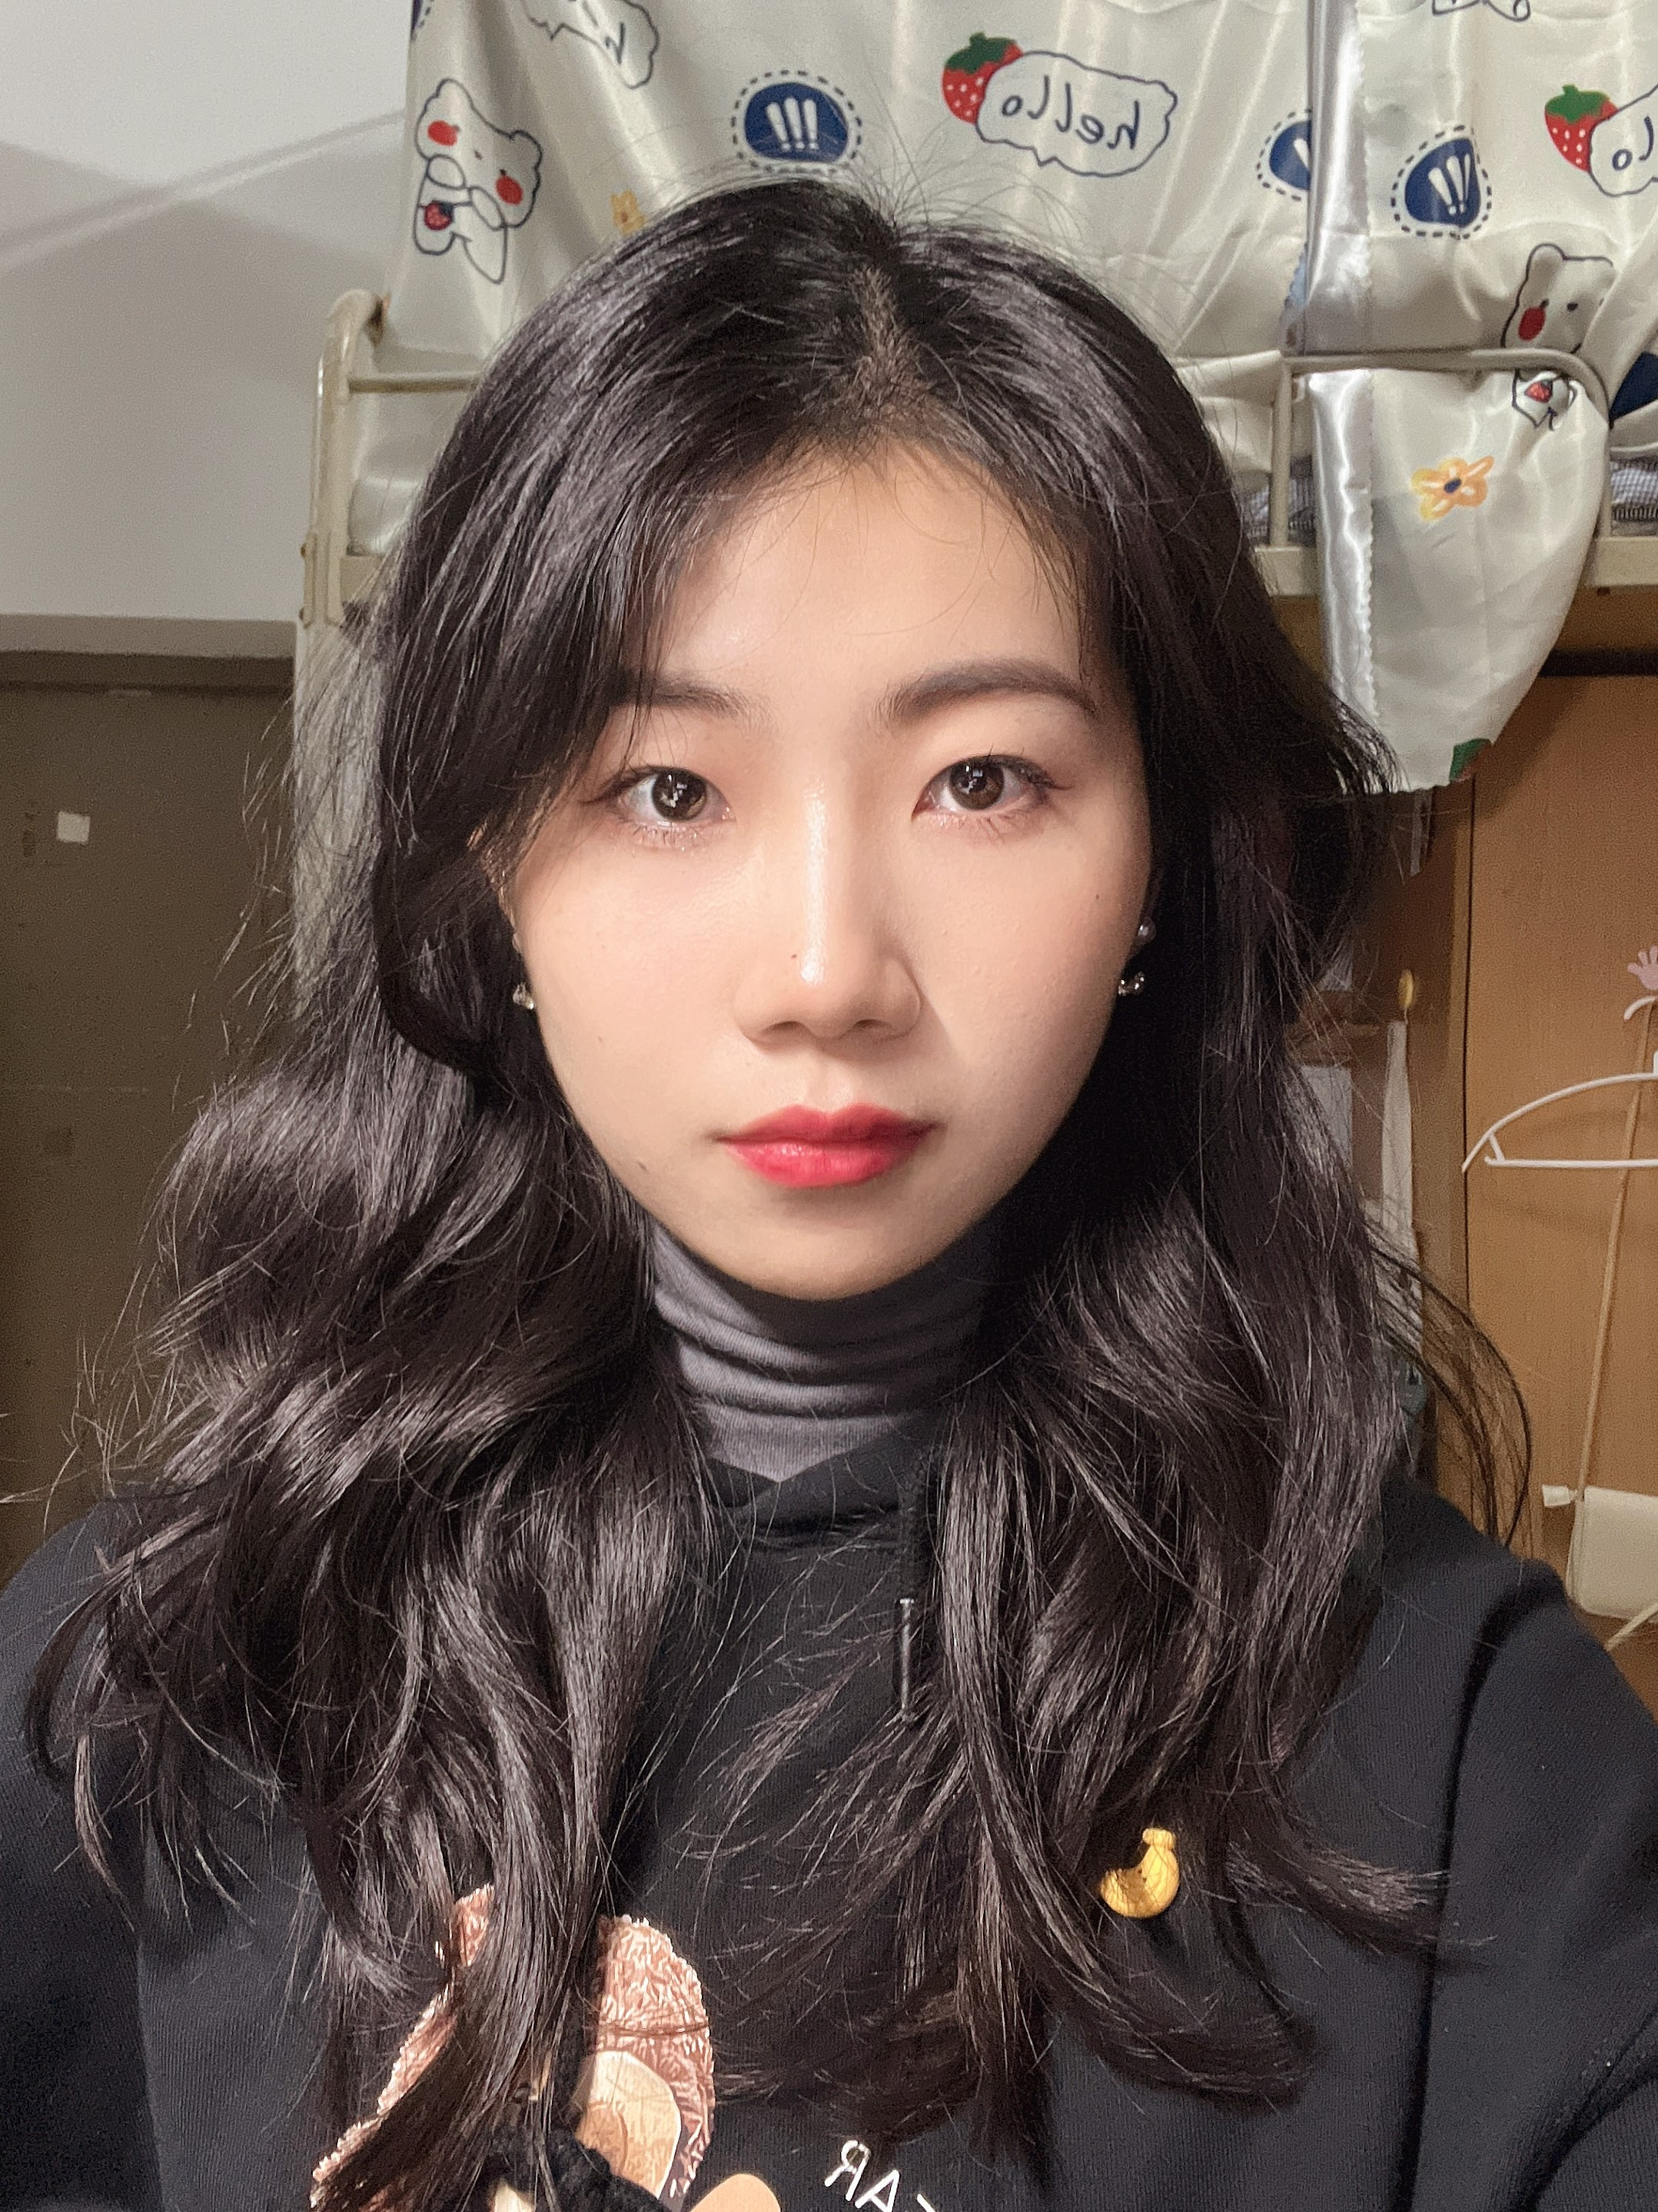
\includegraphics[width=1in,height=1.25in,clip,keepaspectratio]{Fanghan.jpg}}]{Fanghan Yang}
(Postgraduate,~XDU) Received the B.Sc. degree in Artificial Intelligence from the Xidian University, Xi'an, in 2017, and won 2020 American College Students mathematical Modeling Competition Meritorious.Her main research direction is satellite image change detection.

\end{IEEEbiography}


 \begin{IEEEbiography}[{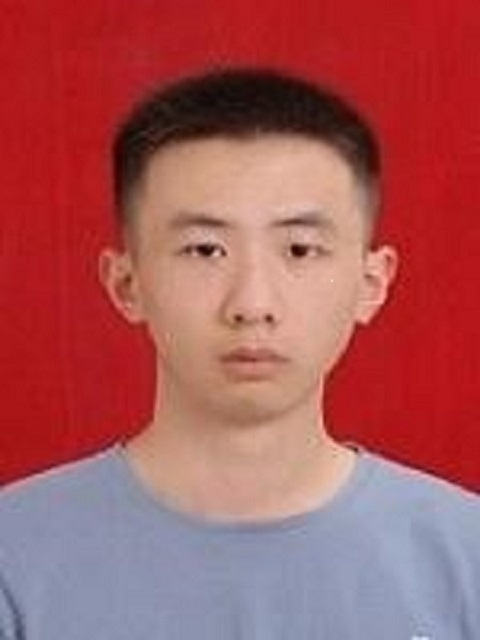
\includegraphics[width=1in,height=1.25in,clip,keepaspectratio]{Zhaoji.jpg}}]{Zhaoji Wu}
(Postgraduate, XDU) received the B.Sc. degree in Artificial Intelligence from the Xidian University, Xi'an, in 2017, and won Provincial first prize in  National College Students Mathematical Modeling Competition. His main research direction is Remote Sening Image Captioning.
\end{IEEEbiography}

  \begin{IEEEbiography}[{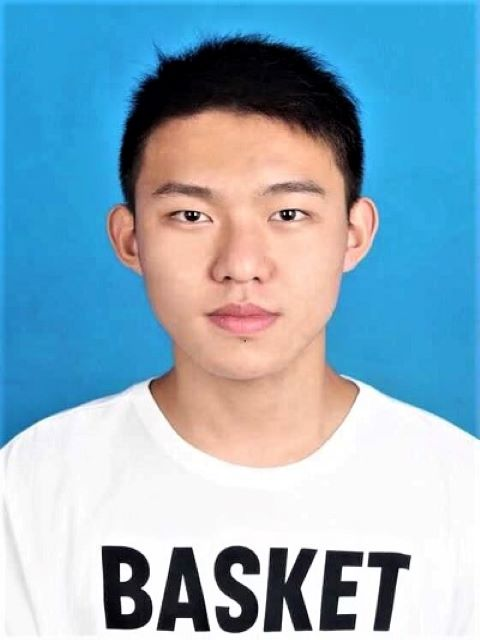
\includegraphics[width=1in,height=1.25in,clip,keepaspectratio]{Xiyu.jpg}}]{Xiyu Fan}
	received the B.Sc. degree in Artificial Intelligence from the Xidian University, Xi’an, in 2017.His current mentor is Xiangrong Zhang, and his main research direction is satellite image object tracking.
 \end{IEEEbiography}

 \begin{IEEEbiography}[{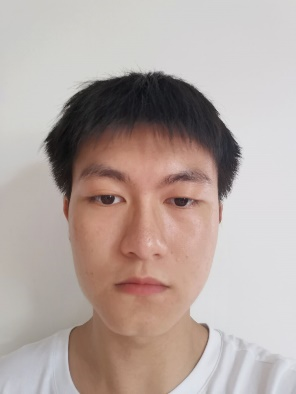
\includegraphics[width=1in,height=1.25in,clip,keepaspectratio]{Zhenhang.jpg}}]{Zhenhang Weng}
(Postgraduate,~XDU)Received a bachelor's degree in Artifificial Intelligence from the Xidian University in 2017, and won the provincial awards of the National College Students' innovation and entrepreneurship training program in 2019.His research interest is remote sensing image processing and analysis.
\end{IEEEbiography}


\end{document}


